% Chapter 2

\chapter{Background Research} % Chapter title

\label{ch:background} % For referencing the chapter elsewhere, use \autoref{ch:background} 

%TC:ignore
%This is the Background chapter, it should be approximately 4,000 Words in total.
%SRAM-PUF section should be approximately 1,500 words longs
%Fuzzy Extractor section should be approximately 1,500 words long.
%Forward error correction subsection should make up approximately 500 words.
%Cryptographic Hashing subsection should be about 500 words long.
%Networking section should be 1000 words in length.
%TC:endignore 
%-------------------------------------------------------------------------------

The intention of this project is to investigate and impliment in whole - or in
part - a prototypical networed device that can be authenticated using a \gls{puf}.
As explained in the Introduction there are three areas under investigation. Below
are the research findings within each of these areas which supported system
design that will be discussed in the next chapter.

\section{PUFs \& SRAM}

The first thing required for a \gls{puf} based authentication system is
obviously, a \gls{puf}.
Introduced in 2002\cite{pappu2002puf}, 
\glspl{puf} can be built from a wide variety of technologies, some have
electronic construction, some not and new designs seems to appear every year.
Of those \glspl{puf} that are created from electronic circuits there are some
that can use off-the-shelf components and some that must be custom made in
silicon. 

\gls{sram} \glspl{puf} that use the meta-stability of the six transistor
\gls{sram} cell (see \ref{fig:sram}) are of the former, were initially proposed by
Guadardo\cite{guajardo2009puf} and are the focus of this project.

\begin{figure}
  \centering
  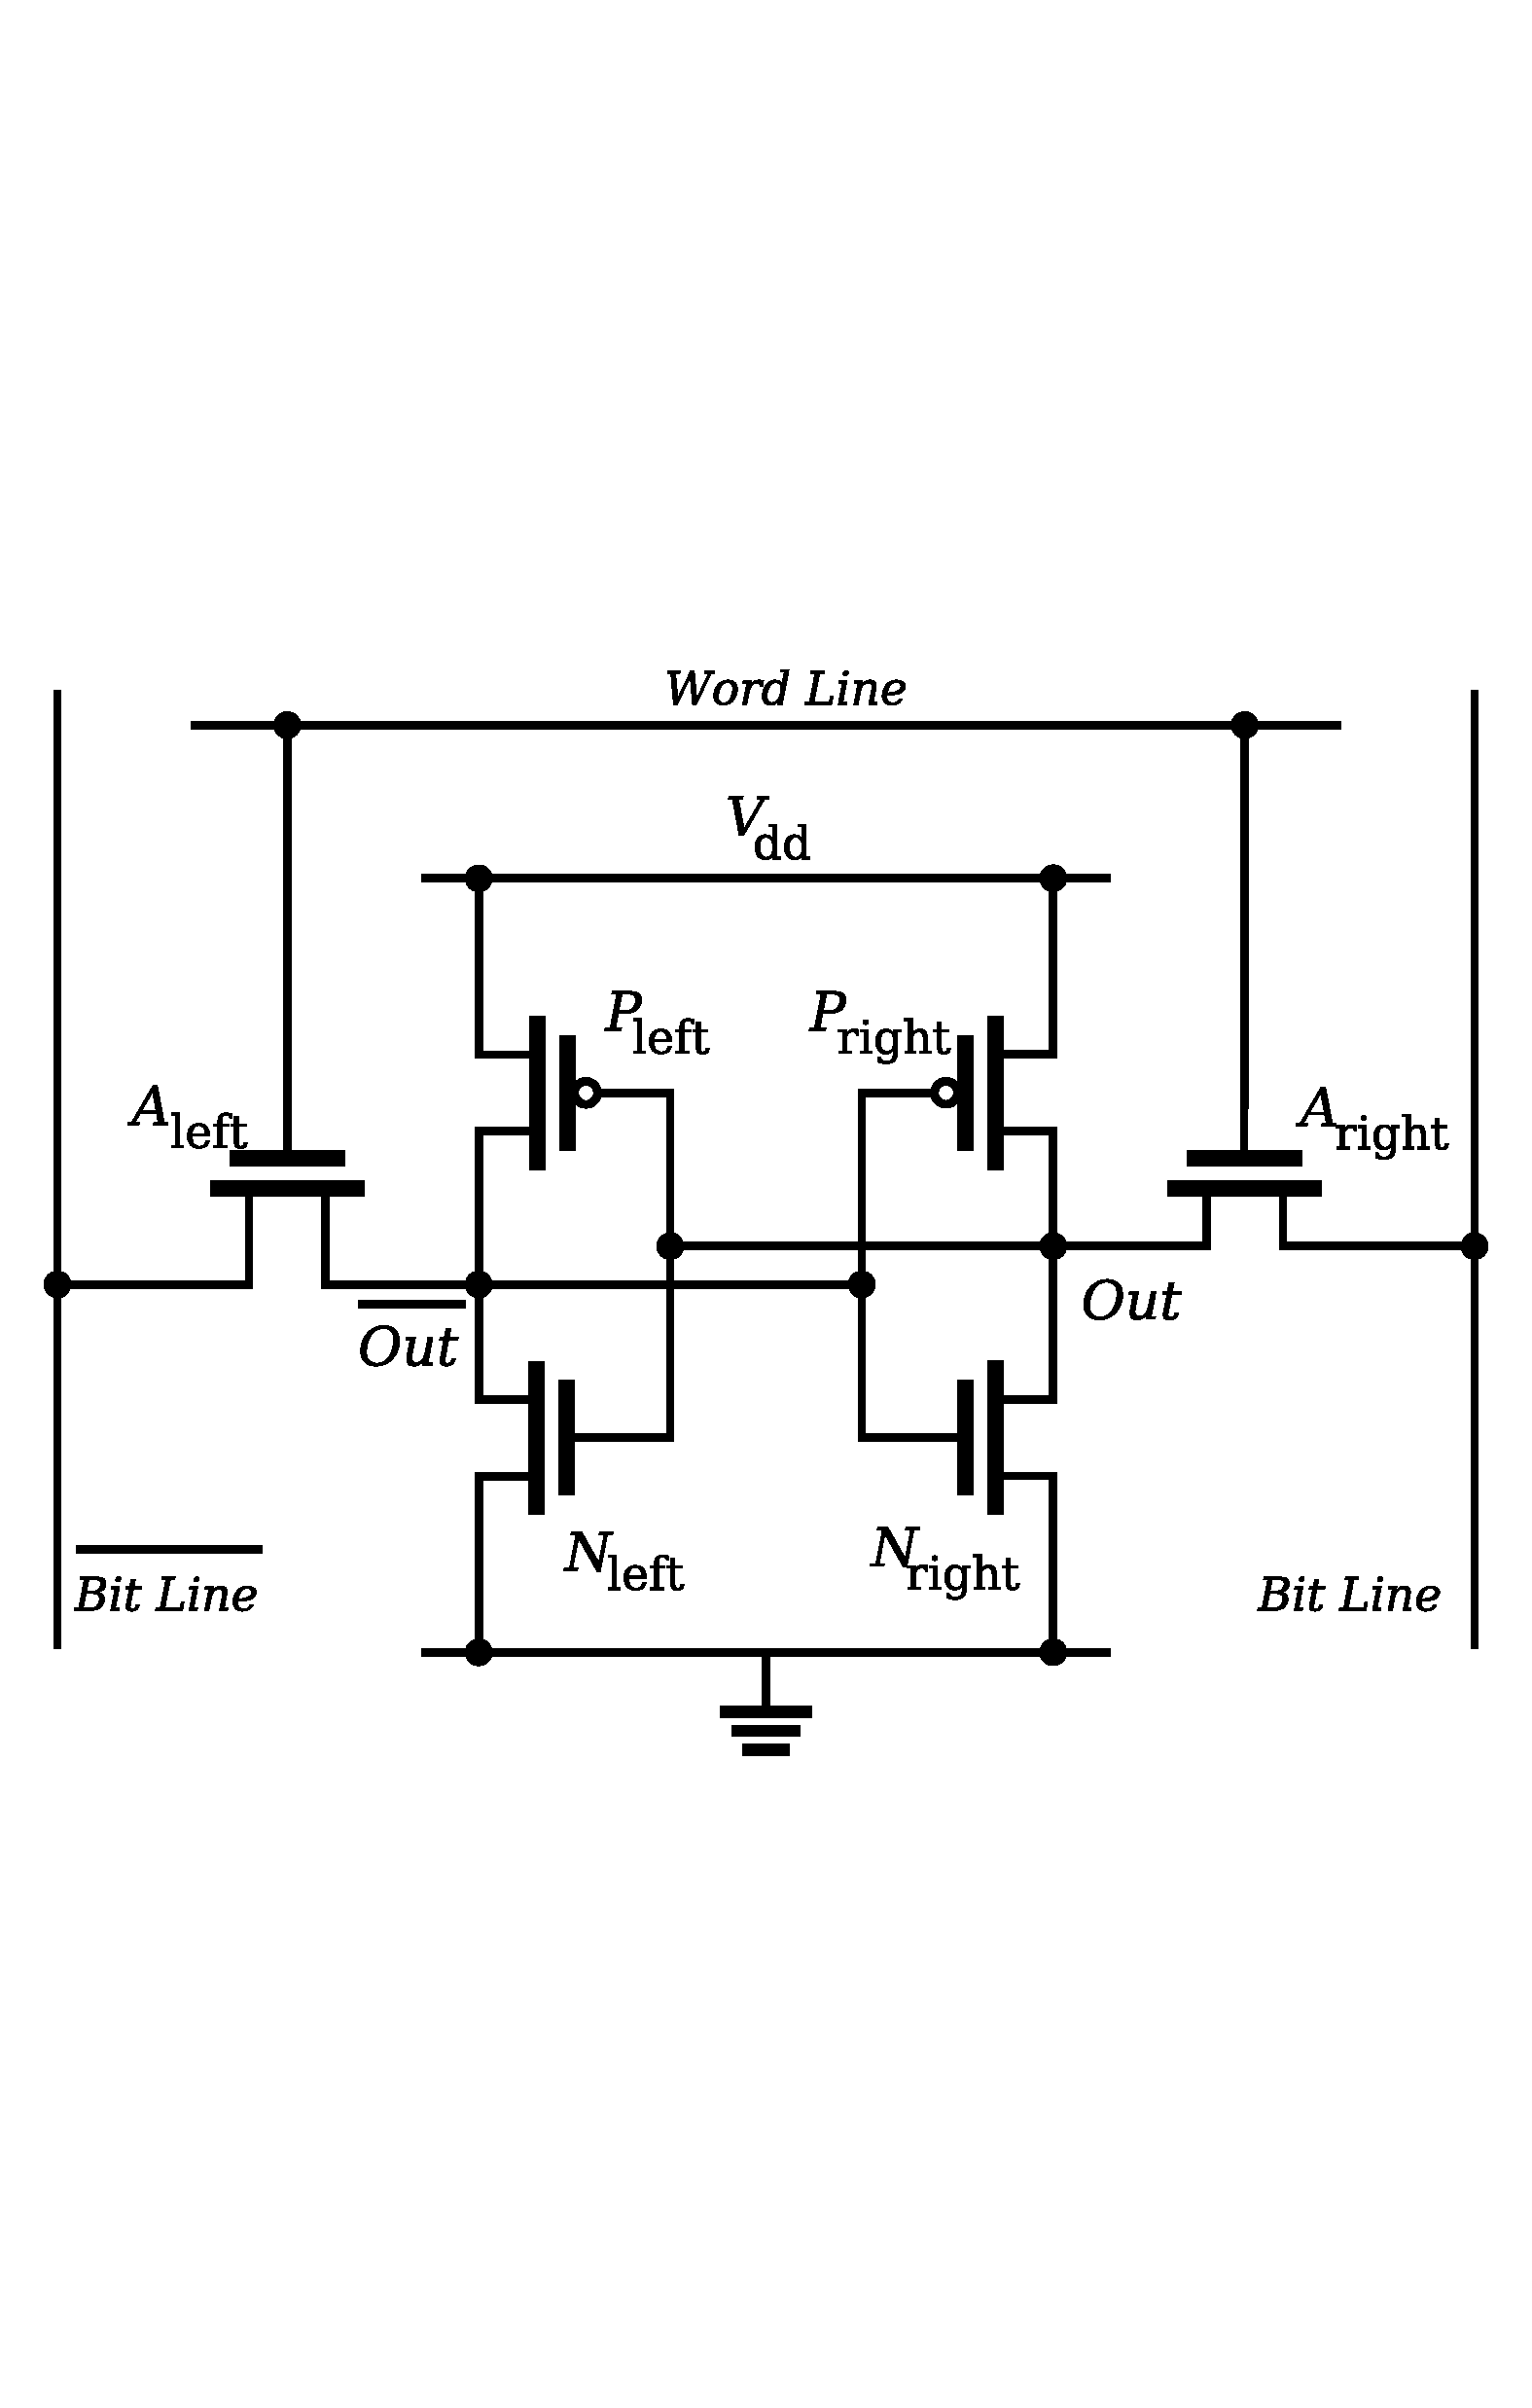
\includegraphics[scale=0.4, trim=0 300 0 300, clip]{images/sram}
  \caption{Six transistor SRAM diagram}
  \label{sram}
\end{figure}

An \gls{sram} cell is conventionally constructed from \glspl{mosfet} in the
ubiquitous, modern photo-lithography process.
Any imperfections in the fabrication of the cell\footnote{such as subtle 
variances in the transistors size, tiny changes in performance
characteristics due to silicon impurities, or any other of minute variance in
any of a thousand manufacturing steps} will result in a cell that is
predisposed to initialise to a particular binary value.
This meta-stability is a central underlying principal for the \glspl{sram}
functionality.

To construct a \gls{sram} based \gls{puf} either the \gls{sram} must be
incorporated into the design of an \gls{ip} core on the \gls{asic} itself,
or it could be access from outside.
In a practical \gls{puf} core of an embedded device the former may be easier
to implement, but the later would take less space.
In the case of this project - where a physical \gls{ip} core will not be
implemented - the functionality is intended to reside in an \gls{fpga},
the acquisition of a separate \gls{sram} device is required as a basic
\glspl{fpga} chip itself is unlikely to have the memory quantity required.
A device that does not have any the property of initialising the memory cell
contents to a set value upon power-up is essential, and the
ability of the \gls{puf} implementation to control the power supply to the 
\gls{sram} device is to be desired.

Unfortunately, in the case of many \gls{fpga} development boards, such as the
Altera DE-1\cite{altera2006usermanual} the \gls{sram} chip on the board itself
is not completely compatible with this usage.
This is because the wire that powers the chip in operation is simply wired to
the required voltage rail of the board.
Without the ability to physically turn the \gls{sram} chip off and back on,
its initial values are available only once, however the simplicity of the
interface and it easy availability make it a good choice for preliminary work
such as that carried out in this project.

\section{Fuzzy Extractors}

\subsection{Introduction}

The way \glspl{puf} are implemented means that their raw
output is often - and perhaps necessarily - \emph{‘fuzzy}’ (or \emph{noisy}).
That is to say that it is far from guaranteed that any individual bit or
symbol within the data extracted from the \gls{puf} will remain the same when checked
again.
This could be due to variations in conditions (such as temperature or \gls{rf} interference) or by degradation or wear of the physical substance that the
\gls{puf} is created out of.
This can be naively solved by accepting some threshold of errors in the response
of the \gls{puf} with respect any particular challenge.
However, this is not efficient and severely limits the cryptographic security
of the device.
It would be far preferable to be able to have some sort of \emph{‘wrapper}’
around the device that corrects the errors internally and can be guaranteed
with some degree of certainty to output the same response to a challenge even
if conditions have changed or the device has degraded over time.

As it turns out, such a wrapper exists. This is called a \textbf{Fuzzy Extractor} which
was first proposed by Dodis et al\cite{dodis2004fuzzy} for handling biometric data for cryptographic situations.
In layman’s terms, this involves three separate processes.
Firstly, and most essentially, a \emph{secure sketch} which extracts and recovers stable
cryptographic key data in a noise tolerant way.
Secondly, a \emph{privacy amplification} process is implemented through a \emph{randomness extractor}.
In more specific terms, this process obscures the key by hashing the initial
output of the secure sketch - which could be quite regular -and increasing its randomness, thus making the message much more difficult for an adversary to break.
In any practical implementation of the two above processes of a Fuzzy extractor,
it is at least necessary to implement one further component; a source of randomness.
This is needed by both others in the generation stage.

These components can be implemented in a variety of ways, but generally the secure sketch requires the implementation of some kind of \gls{ecc}.
The randomness extractor requires the implementation of a cryptographic hash
function. and the source of randomness needs to be practically non-deterministic.

\subsubsection{Source of Randomness}
Randomness can be sourced from the implementation of a \gls{rng}.
Many different types have been proposed in the literature and can be separated
into two classes, \glspl{trng} and \glspl{prng}.
The difference being that true randomness requires sampling
from a noisy physical process and are (in theory) completely unpredictable.
Pseudo random number generators are deterministic, and as such can be considered a mathematical function which can be replicated by an attacker.
Thus, it is far more secure to use a true random number generator if possible.

On an \gls{fpga}, a relatively easy way to implement a \gls{trng} is by
the sampling of one internal/external clock of the device at periods controlled
by an independent clock.
Due to the slight variances in each clocks’ rate (based on their individual
underlying physical implementations) it is undeterminable
whether a clock will be high or low when it is sampled.

Implementing this on a \gls{fpga} was attempted but not completed, and so a
\matlab simulation was employed for this purpose.

\subsection{Secure Sketch with BCH encoding}

\Glspl{ecc}, in simple terms, use extra redundant information to
provide a scheme for some number of errors in a message to be detected and
eliminated. Generally these have been most usefully applied in the field of
network communications. In the fuzzy extractor, this ability to correct errors
can similarly be used to eliminate inherent noise to produce cryptographic key
data with a high probability of correctness. This is exactly what is needed for
implementation of the secure sketch process.

There are many types of error-correcting code, some more suitable in the
implementation of a fuzzy extractor than others, especially when implementing
for embedded devices where electronic complexity needs to be minimised.
The theory of error-correcting codes is often introduced by the Hamming code.
This most simple of codes can be generalised as a cyclic linear block code.

Block codes, as opposed to convolutional codes such as the Viterbi algorithm,
work on fixed sized packets of symbols rather than streams of data. The raw data
coming out of the \gls{puf} is of a fixed size, therefore block codes are the obvious
choice for implementing a secure sketch. However, Hamming codes can only correct
one error, the raw output of a PUF could potentially contain more than one
error, and therefore it is necessary to explore other schemes. 
 
BCH Codes where first proposed by Alexis Hocquenghem, and independently Raj Bose
and D. K. Ray-Chaudhuri (the name ‘BCH’ being an acronym of their surnames).
It is a type of cyclic linear block error-correcting code. They historically
build upon, and can be seen as a generalisation and refinement of, the Hamming
codes proposed by Richard Hamming in 1950. BCH codes are binary in the nature
of their symbols, unlike other block codes such as the more famous Reed-Solomon
code used for error-correction for compact discs. This binary nature allows for
a more compact implementation in embedded hardware and is easier to implement
in \gls{vhdl}.

Again, Implementation of complimentary BCH Encoder and Decoder in \gls{fpga} was
looked at, but for reasons of expediency this was not completed, and a \matlab
simulation was used.

\subsection{Privacy Amplification with SHA-256}

Hash functions are any function that maps variably sized input data (message) to
output data (the hash, or message digest) of a fixed size. They are primarily
used in hash tables to speed up data searches. However, they have a wide variety
of other uses such as use in cryptography. A cryptographic hash function can be
defined as any hash function where it is infeasible to generate the input given
the output, i.e. it is impossible to invert the function in a practical sense.

In finding a suitable cryptographic hash function for privacy amplification
purposes there are also three other properties that it would be ideal for it to
have. These are; that it is simple to implement the hash algorithm, that the
likelihood of finding two different inputs that map to the same output data is
microscopically small (collision resistant) and finally it is practically
impossible to generate the required input data for a given output data (one-way
function or pre-image resistant).

Such cryptographic hash functions are widely suggested in the literature.
However, in the context of an embedded system, a balanced compromise between
the cryptographic strength of the hash function and the complexity of its
implementation is paramount.  Rigorously assessing the cryptographic security
of a hash deceptively difficult and beyond the scope of this project.
Therefore, implementation an original hashing scheme would be ill-advised.
It is far better to tailor an existing and well-understood and tested scheme
for the purpose.

The standard cryptographic hash function set called SHA-2.
\gls{sha2} was designed by the \gls{nsa} in 2001.
It avoids some flaws in its predecessor SHA-1, yet is relatively simple
to implement in hardware. The set consists of hash functions differentiated by
their digest size (224, 256, 384, and 512 bits). They all operate using a
similar structure, but for easy implementation in \gls{vhdl} the 256-bit
implementation (SHA-256) is the most appropriate choice as it is one of the
smallest and the digest size is a power of two, which is often beneficial in
simplifing hardware implementations.


\section{PUF Enhanced Network Authentication Protocols}

In providing a \gls{puf} authentication mechanism thought should be first given
to where in the protocol stack would be most effective. For an embedded device
a high layer such as the applications or session layers of the OSI model would
seem both inefficient and unnecessary. Going done the stack, it would also seem
that establishment of the transport and network levels presupposes the device
has already obtained access to a point-to-point connection or \gls{lan}. This
would suggest a suitable place to establish authentication through \gls{puf} is
at the data link layer.

The link layer consists of both direct connection protocols involving only two
devices such as \gls{slip} and \gls{ppp} and multi-node protocols where the
communication channel is shared such as Ethernet and Wi-Fi. In invisioning a
future 'Internet-of-Things' protocol reling on \glspl{puf} it would seem
advisable to look a the multi-node protocols, specifically those for wireless
networking.
However in attempting to keep the project focused it would be preferable to
investigate procotols in a simplier setting. Thus a compromise of investigation
of modifications to the Ethernet protocol was reached.

Any modern link-layer network authentication system that is intended to
replace or improve upon current standards in the most part necessitates
adhering to much the same high security methods utilized in modern cryptographic
protocols such as  \gls{wpa} and more recently \gls{wpa2} in Wireless protocols.
This is because those methods have been both proved secure through exposure to
the 'real-world' and provision for those methods is readily available to
industry. Modern standards such as \gls{wpa2} and gls{pppoe} all support the use
of .. for security provision at the data link layer employ
the \gls{eap} framework. The underlying authentication methods is encapsulated
by \gls{eap} which provides for the safe transfer of any parameters and secret
key information for the method itself.

\Gls{eap} can be utilised over Ethernet using the ISO/IEC/IEEE standard
802.1X\cite{8802-1x} and it uses the standard Ethernet packet format with a
\emph{EtherType} set to the value \inlinecode{0x888E}.
The idea is that those devices requiring authentication to the network knwon as
/emph{supplicants} are not allowed to send Ethernet packets of any other 
EtherType, including general ones such as \inlinecode{0x0800} IPv4 Packets.
Thus a attacking device can do no harm to any other device on the network -
every attempt to communicate will be dropped until authenticated.

In the case of Ethernet 

Paramount to the issue of running out of keying data for a protocol given the ultimately finite nature of \gls{sram} memory and therefore the finite number of challenges that can be made without repeating the data - a fundemental issue in cryptpography. 

In utilizing a \gls{puf} in 

As the digest output of hash function is the ultimate response of the device
to a challenge this means that the response size is 256-bits or 32 octets.
This is half the minimum required packet payload size.